\section{Splitting of femoral cartilage volume for meshes}
\label{sec:Splitting}
As described above, constructing meshes for the femoral cartilage is not possible without some pre-processing. The convex parts of the volume on either side need to be split off and rotated by 90° so that minimum and maximum points can reliably be extracted without missing a significant amount. The sections are isolated as follows: 
\par\noindent
The cartilage volume is a point cloud made up of vectors $(x, y, z)$. Group the points by $(x, y)$ and for each of these combinations, calculate the range of $z$. Then calculate the mean or median of $z$ and take all combinations $(x, y)$ for which the range of z is less than the previously calculated mean/median, i.e. those points where the minimum and maximum z values are not too far apart. Note that the convex parts of the cartilage are characterized by a large ranges for z. Having now isolated the central part of the volume, it is a trivial task to extract the convex parts: We can calculate the minimum and maximum x value of the central vectors, and everything left of the minimum gets assigned to the left convex part, and everything right of the maximum gets assigned to the right convex part.
\par\noindent
With the sections isolated, the problematic convex parts can then be rotated by 90°. Now, again for every combination $(x, y)$, the vector $(x, y, max(z))$ can be added to the upper mesh, and the vector $(x, y, min(z))$ to the lower ($min(z)$/$max(z)$ may be replaced by distance to a central point, depending on implementation).

\begin{minted}[escapeinside=~~,mathescape=true,breaklines,linenos]{text}
	Procedure to split a femoral cartilage volume into three parts
	Given:
	volume := vectors (x, y, z) making up the volume
	
	Procedure:
	z_range := volume.group_by((x, y)).z.max() - volume.group_by((x, y)).z.min()
	z_med := median(z_range)
	z_index := {d ~$\in$~ volume | d.z < z_med}
	lower_bound := {min(d.x) | d ~$\in$~ z_index}
	upper_bound := {max(d.x) | d ~$\in$~ z_index}
	left_part := {d ~$\in$~ volume | d.x < lower_bound}
	middle_part := {d ~$\in$~ volume | lower_bound < d.x < upper_bound}
	right_part := {d ~$\in$~ volume | d.x > upper_bound}
	left_part := rotate(90)
	right_part := rotate(90)
\end{minted} 

\begin{figure}[htb!]
	\centering
	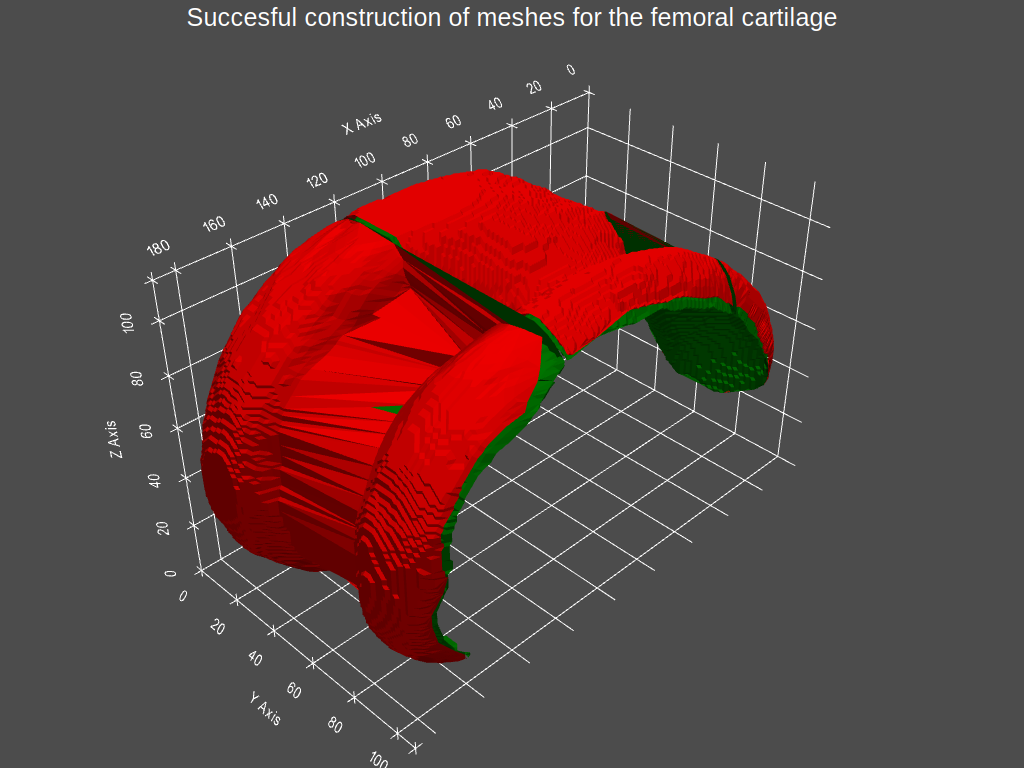
\includegraphics[width=\linewidth]{./figures/femoral_meshes}
	\caption{Successful construction of meshes for the femoral cartilage}
	\label{fig:femoral_meshes}
\end{figure}